\chapter{BÀI TOÁN HỆ THỐNG GỢI Ý}
\section{Giới thiệu bài toán}
\subsection{Vấn đề đặt ra}
Trong thế giới ngày nay, với sự phát triển vượt bậc của nền văn minh nhân loại, công nghệ có nhiều những đột phá mới, con người được hưởng lợi từ sự hiện đại hóa của xã hội. Những công nghệ mới được sản sinh ra để phục vụ cho những tiện ích của con người, với sự bùng nổ của mạng internet những năm vừa qua, các nền tảng mạng xã hội trực tuyến cùng với đó cũng kéo theo những vấn đề xung quanh nó. Con người hiện đại ưa chuộng các hình thức mua sắm trực tuyến vì sự tiện lợi và dễ dàng sử dụng. Một vấn đề đặt ra làm sao đưa đến thông tin sản phẩm phù hợp với người dùng. Tức chúng ta cần gợi ý cho người dùng những sản phẩm phù hợp với họ, để họ có thể dễ dàng tiếp cận và sử dụng từ đó nâng cao doanh số của các của hàng cũng như là khách hàng có thể được sử dụng loại sản phẩm mà họ yêu thích.\\
Các cửa hàng truyền thống, để thu hút được khách hàng, họ thường trưng bày các sản phẩm đang được ưa thích hoặc phổ biến trên thị trường để tạo ấn tượng với khách hàng, và các sản phẩm ít được phổ biến hơn thì họ thường cất trong kho, hoặc không để ra trưng bày. Với cách làm đó thì những sản phầm được trưng bày ra chưa chắc đã phù hợp với người mua, còn những sản phẩm không được trưng bày thì có thể phù hợp khách hàng nhưng họ lại không tìm thấy sản phẩm. Đó là một hạn chế với những cửa hàng truyền thống khi họ không thể trưng bày tất cả sản phẩm của họ. Nhưng đối với các cửa hàng trực tuyến thì tất cả sản phẩm của họ được đưa đến với người dùng những thông tin đầy đủ nhất. Và khi mà lượng thông tin về các sản phẩm quá nhiều, làm cho người dùng không biết nên lựa chọn sản phẩm nào thì lúc này một vấn để xảy ra là làm thế nào có thể gợi ý cho người dùng những sản phẩm mà phù hợp với họ nhất. Lúc này những ý tưởng về bài toán gợi ý đã ra đời và mang lại những hiệu quả nhất định, giúp cho những công ty có thể tăng doanh số của mình. Hệ thống gợi ý là công cụ lọc thông tin mạnh mẽ có thể thúc đẩy các dịch vụ cá nhân hóa và cung cấp trải nghiệm riêng biệt cho từng người dùng. Nói ngắn gọn, hệ thống đề xuất đóng vai trò nòng cốt trong việc tận dụng nguồn dữ liệu dồi dào hiện có để giúp việc đưa ra lựa chọn dễ dàng hơn.
\begin{center}
    \begin{figure}[H]
    \begin{center}
     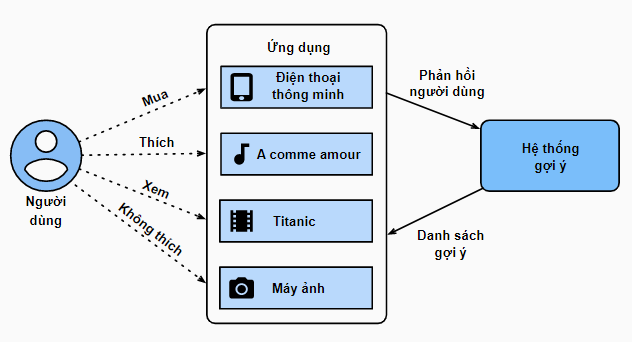
\includegraphics[scale=.8]{images/Screenshot 2022-07-17 172951.png}
    \end{center}
    \caption{Minh họa cho quá trình gợi ý.}
    \label{refhinh1}
    \end{figure}
\end{center}

\subsection{Mô hình hóa bài toán}
Như đã đề cập, những dữ liệu trong bài toán của chúng ta là thông tin người dùng, thông tin sản phẩm, và một chỉ số thể hiện người dùng có quan tâm đến sản phẩm đó hay không. Ta có biến $user$ thể hiện cho người dùng, $item$ thể hiện cho sản phẩm, và một chỉ số đo mức độ quan tâm của $user$ với $item$ là $rating$, ta có thể hiểu đó là đánh giá của người dùng cho sản phẩm đó.\\
Từ các khái niệm đó ta có được một ma trận tiện ích (Utility matrix) là tập hợp tất cả $rating$ của tất cả người dùng với tất cả sản phẩm, kể cả các $rating$ chưa biết.
\begin{table}[H]
\centering
    \begin{tabular}{|c|c|c|c|c|c|}
\hline
     &user\_1 & user\_2& user\_3& user\_4& user\_5  \\ \hline
     item\_1& 1& 4& 3 & 5& 2 \\ \hline
     item\_2& 5& ?& ? & 3& ? \\ \hline
     item\_3& 0& 4& ? & 2& 2 \\ \hline
     item\_4& ?& 4& ? & 1& 2 \\ \hline
\end{tabular}
\caption{Ma trận tiện ích (Utility matrix)}
\end{table}
Đây là ví dụ về ma trận tiện ích có 5 $user$ và 4 $item$ và các $rating$ tương ứng, ở đây ta thấy có một số $rating$ chưa được người dùng đánh giá sản phẩm và để ở trạng thái dấu "?". Công việc của ta là dự đoán các $rating$ đó để đoán xem người dùng có quan tâm đến sản phẩm đó hay không để gợi ý cho họ. Hay nói cách khác bài toán của chúng ta là đang đi điền các giá trị "?" để hoàn thành ma trận.\\
Trong thực tế, ta có rất nhiều các $user$ và $item$ nhưng lượng $rating$ lại rất ít, vì người dùng thường chỉ đánh giá một số ít các sản phẩm mà họ đã mua, vì thế ma trận Utility thường có rất nhiều giá trị chưa biết. Điều đó làm cho việc dự đoán các giá trị này trở nên khó khăn hơn.\\
Khi lượng người dùng đánh giá nhiều hơn trên các sản phẩm, sẽ làm cho mô hình của chúng ta dự đoán chính xác hơn. Vì thế các hệ thống bán hàng luôn mong muốn các khách hàng có thể đánh giá sản phẩm của mình để có thêm nhiều thông tin hơn.
\subsection{Một số kĩ thuật trong hệ thống gợi ý}
Có rất nhiều thuật toán dùng trong hệ thống gợi ý với đầu vào là sự đánh giá của người dùng trên một số sản phầm, và sinh ra một danh sách các sản phẩm gợi ý cho họ. Một số có đầu vào là toàn bộ hành vi, nhận xét, đánh giá của người dùng để đưa ra mức độ dự đoán chính xác nhất.\\
Có 3 kĩ thuật phổ biến thường được nhắc đến khi sử dụng trong hệ thống gợi ý là Lọc dựa trên nội dung (Content–Based Filtering - CBF), Lọc cộng tác (Collaborative Filtering - CF) và Lọc nhân khẩu học (Demographic Filtering - DF).\\
Ta định nghĩa tập $U$ là tập các người dùng, $u \in U$ với $u$ là người dùng thuộc tập $U$. Tập $I$ là tập các sản phẩm, $i \in I$ với $i$ là sản phẩm thuộc $I$.
\begin{table}[H]
    \centering
    \begin{tabular}{|p{3cm}|p{3cm}|p{3cm}|p{3.5cm}|}
    \hline
        \textbf{Kĩ thuật} & \textbf{Tổng quát}& \textbf{Đầu vào}& \textbf{Quá trình} \\ \hline
         Collaborative & Các đánh giá của $U$ đến $I$ & Các đánh giá của $u$ đến $I$ & Xác định các $user$ trong $U$ giống với $u$ và suy ra đánh giá  của họ với $item$ $i$.\\ \hline
         Content-based & Đặc trưng của các $item$ thuộc $I$ & Đánh giá của $user$ $u$ lên các $item$ trong $I$ & Tạo một bộ phân loại phù hợp với hành vi xếp hạng của u và sử dụng nó trên $i$.\\ \hline
         Demographic & Thông tin nhân khẩu học về $U$ và xếp hạng của họ đối với các mặt hàng trong $I$ & Thông tin nhân khẩu học về $u$ & Xác định những $user$ tương tự về mặt nhân khẩu học với $u$ và suy ra xếp hạng của họ về $i$. \\ \hline
    \end{tabular}
    \caption{Các kĩ thuật trong Recommendation System.}
    \label{tab:my_label}
\end{table}

\subsubsection{Lọc cộng tác - Collaborative Filtering (CF)}
Trong kĩ thuật này, hệ thống dựa vào sự tương quan giữa các người dùng với nhau, các người dùng có sở thích, đánh giá gần giống nhau khả năng cao họ sẽ có đánh giá giống nhau ở một sản phẩm khác. Khi đó $user\_i$ đánh giá tốt một $item\_j$ thì hệ thống sẽ gợi ý $item\_j$ đó cho những $user$ khác có tương quan cao với $user\_i$.\\
Đã có nhiều hệ thống gợi ý sử dụng kĩ thuật này trong môi trường kinh doanh hoặc trong môi trường học thuật, nó vẫn rất hữu ích. Vấn đề với CF là chúng chỉ hoạt động tốt nhất khi số lượng mặt hàng được đánh giá trên mỗi người dùng cao và các vấn đề với người dùng mới và sản phẩm mới chưa được người dùng đánh giá khi có nhiều mặt hàng để xếp hạng, sự cố có thể xảy ra là sự thưa thớt dữ liệu cản trở việc tìm kiếm người dùng tương tự như người dùng mục tiêu.
\subsubsection{Lọc dựa trên nội dung - Content Based Filtering (CBF)}
Cách tiếp cận này yêu cầu việc sắp xếp các sản phẩm vào từng nhóm hoặc đi tìm các đặc trưng của từng sản phẩm. Các sản phẩm có mức tương tự cao về nội dung sẽ được nhóm lại.  Hệ thống sẽ học để gợi ý những sản phẩm mà tương tự với những cái mà người dùng đã thích trong quá khứ. Độ tương tự giữa các sản phẩm được tính dựa trên những đặc trưng kết hợp với những sản phẩm được so sánh.
\subsubsection{Lọc nhân khẩu học - Demographic Filtering (DF)}
Hệ thống gợi ý dựa vào kĩ thuật DF phân loại người dùng theo thông tin nhân khẩu học của họ và gợi ý những sản phẩm phù hợp. Trong DF, hồ sơ người dùng được tạo bằng cách phân loại người dùng theo các mô tả khuôn mẫu, đại diện cho các đặc trưng của các lớp người dùng. Thông tin nhân khẩu học xác định những người dùng thích các sản phẩm liên quan. DF tạo ra các danh mục người dùng có đặc điểm nhân khẩu học tương tự và sau đó hành vi hoặc sở thích mua tích lũy của người dùng trong các danh mục này sẽ được theo dõi. Đối với người dùng mới, các đề xuất được đưa ra trước tiên bằng cách tìm ra danh mục mà người dùng này thuộc vào và sau đó sở thích mua tích lũy của những người dùng trước đó được áp dụng cho danh mục mà người dùng này thuộc về.\\
Giống như các kỹ thuật lọc cộng tác, các kỹ thuật nhân khẩu học cũng hình thành các mối tương quan “people-to-people” nhưng sử dụng dữ liệu không giống nhau.
\section{Kĩ thuật Collaborative Filtering (CF)}
Như đã đề cập ở trên, hệ thống gợi ý dựa trên trên các phương pháp lọc cộng tác dựa trên thu thập và phân tích một lượng lớn thông tin về xếp hạng của người dùng và tạo các gợi ý mới dựa trên các hoạt động so sánh giữa những người dùng và dự đoán những gì người dùng sẽ thích dựa trên sự giống nhau của họ với người dùng khác. CF dựa trên giả thuyết rằng những người đồng ý trong quá khứ cũng sẽ có cùng quan điểm trong tương lai và rằng họ sẽ thích các loại liên quan đến các mặt hàng họ thích trong quá khứ.\\
Hai hướng phát triển chính của kĩ thuật này là \textit{neighborhood methods} và \textit{latent factor models}. Trong đó:
\begin{itemize}
    \item Phương pháp "Neighborhood" tập trung vào việc tính toán các mối quan hệ giữa các $item$ hoặc giữa những $user$. Dựa vào cách tiếp cận sự tương quan giữa các $item$, "item-item", hệ thống sẽ đánh giá mức độ ưa thích của một $user$ đối với một $item$ dựa vào những $item$ khác có độ tương quan gần nhất với $item$ đó mà $user$ đã đánh giá trong quá khứ. Dựa vào cách tiếp cận sự tương quan giữa các $user$, "user-user", khi đánh giá mức độ ưa thích của một $user$ với một $item$ dựa vào việc những $user$ khác có sự tương quan đã từng đánh giá cùng $item$ đó trong quá khứ.
    \item Phương pháp "Latent factor" là một cách tiếp cận thay thế cố gắng giải thích đánh giá bằng cách mô tả đặc điểm của cả $item$ và $user$, chẳng hạn như 20 đến 100 yếu tố được suy ra từ các đánh giá mẫu. Tức là với mô hình này, hệ thống gợi ý đang cố gắng đi tìm hiểu những nhân tố ẩn bên trong những đánh giá của người dùng. Vì những nhân tố ẩn này có thể có tác động nhiều đến sự đánh giá của người dùng lên các sản phẩm mà bằng các độ đo thông thường ta không thể khám phá ra.
\end{itemize} 
Các kĩ thuật CF cũng vẫn tồn tại nhiều thử thách trong thực tế có thể kể đến như dữ liệu thưa thớt, vấn đề về sự xuất hiện các các người dùng mới, hay là những sản phẩm mới, tính ổn định trong việc dự đoán. Những vấn đề đó được liệt kê ở phía dưới một cách chi tiết hơn:
\begin{enumerate}
    \item \textbf{Dữ liệu thưa thớt (Data Sparsity)}: Trong thực tế thì những người dùng thường rất ít đánh giá các sản phẩm mà họ đã dùng, điều đó khiến rất nhiều điểm đánh giá bị thiếu trong ma trận tiện ích, và ma trận trở thành một ma trận thưa. Việc người dùng có ít các đánh giá sẽ làm cho kết quả dự đoán trở nên không đáng tin cậy. Để khắc phục vấn đề dữ liệu thưa thớt, cách tiếp cận được để xuất đó là cố gắng tìm ra một độ đo tương tự mới và sử dụng cho K - Neighbour để dự đoán.
    \item \textbf{Cold Start}: Vấn đề "Cold Start" xảy ra khi trong hệ thống của chúng ta xuất hiện những người dùng mới, sản phẩm mới. Khi đó hệ thống gợi ý hoàn toàn chưa biết về những người dùng mới hoặc sản phẩm mới này, do đó việc dự đoán trở nên không đáng tin. Một số cách giải quyết có thể sử dụng đến như thừa số hóa hàm, xác suất.
    \item \textbf{Drift}: Đây là kết quả một số yếu tố khiến người dùng thay đổi tâm trạng của họ khi đánh giá. Tức là các sản phẩm, hoặc người dùng sẽ thay đổi theo xu hướng thời gian, điều đó làm cho cách đánh giá sản phẩm của người dùng cũng thay đổi theo. Bằng phương pháp học máy ta có thể cho hệ thống học được cả các trọng số thể hiện sự thay đổi này, giúp việc trích xuất hành vi và sở thích của người dùng theo thời gian thích hợp.
    \item \textbf{Khả năng mở rộng}: Sự quá tải của thông tin người dùng và sản phẩm sẽ làm tăng độ phức tạp tính toán. Một số cách tiếp cận để cải thiện khả năng mở rộng của bài toán như phân cụm. 
\end{enumerate}
\section{Phương pháp Matrix factorization}
Cách tiếp cận bằng việc đi khám phá các nhân tố ẩn bên trong ma trận tiện tích được lựa chọn phổ biến và đạt được sự thành công dựa trên phương pháp phân tích ma trận thành nhân tử (Matrix factorization - MF).\\
\subsection{Mô hình Matrix factorization}
Để biểu diễn những nhân tố ẩn quyết định đến sự đánh giá của người dùng bên trong $item\_i$, ta định nghĩa vector $q_i \in \mathbb{R}^f$, và định nghĩa các nhân tố tiềm ẩn bên trong người dùng $u$ là vector $p_u \in \mathbb{R}^f$.
Đối với $item$ $i$ nó sẽ mang nhân tố ẩn ở một mức độ nào đó được thể hiện trong các hệ số tương ứng trong vector $q_i$, có thể là tiêu cực hoặc tích cực. Tương tự với mỗi $user$ $u$ các yếu tố của $p_u$ đo lường mức độ quan tâm của người dùng đối với các mặt hàng trên các yếu tố ẩn tương ứng. Và kết quả của phép nhân 2 vector $q_i ^T p_u$ là kết quả đánh giá của $user$ $u$ lên $item$ $i$. Để dự đoán cho các $rating$ bị thiếu trong ma trận tiện tích, kí hiệu  $\hat r_{ui}$ là các giá trị đánh giá còn thiếu của $user$ $u$ đối với $item$ $i$, được tính như sau:
\begin{center}
    \begin{equation}
        \hat r_{ui} = q_i ^T p_u
    \end{equation}
\end{center}
Bằng cách học từ dữ liệu ta sẽ tìm các $q_i$ và $p_u$ xấp xỉ được gần nhất với các giá trị còn thiếu trong ma trận tiện ích.\\
Bài toán của chúng ta có $m$ sản phẩm, $n$  người dùng, do đó ma trận tiện ích $U$ có kích cỡ là $m \times n$.\\ 
Với $m$ $item$ ta sẽ có được ma trận chứa các nhân tố ẩn của các $item$ là $Q_{f \times m}$, đối với $n$ $user$ ta có ma trận $P_{f\times n}$. Số $f$ ở đây chính là số các nhân tố tiềm ẩn.\\
Mô hình hóa dưới dạng các ma trận ta có:
\begin{center}
    \begin{equation}
        U \approx \hat U = Q^TP
    \end{equation}
\end{center}
Bằng cách này ta đang đi tìm một xấp xỉ ma trận $U$ bằng tích 2 ma trận $Q \in \mathbb{R}^{f \times m}$ và ma trận $P \in \mathbb{R}^{f \times n}$. Thông thường ta chọn $f$ là số nhỏ hơn rất nhiều so với $m,n$.
\subsection{Hàm mất mát (Loss function)}
Để tính lỗi cho các giá trị dự đoán, ta dựa vào phương pháp bình phương cực tiêu. Mục đích của ta là đi tối thiểu sai số giữa giá trị đúng và giá trị dự đoán:
\begin{center}
    \begin{equation} \label{lossfunc}
        \min \mathop {L}\limits_{q*,p*}= \frac{1}{{2k}}\sum\limits_{(u,i) \in K} {{{({r_{ui}} - q_i^T{p_u})}^2} + \frac{\lambda}{2} ({{\left\| {{q_i}} \right\|}^2} + {{\left\| p_u \right\|}^2})}
    \end{equation}
\end{center}
Ta có $K$ là tập các cặp $(u,i)$ mà ta đã biết giá trị đánh giá $r_{ui}$ hay chính là tập training của chúng ta, $k$ là số phần tử tập $K$. Thành phần thứ nhất là trung bình sai số của mô hình, thành phần thứ hai chính là regularized giúp cho mô hình tránh được việc học quá khớp (hiện tượng overfitting). $\lambda$ là siêu tham số. ${{{\left\| {{q_i}} \right\|}^2}}$ và ${{{\left\| p_u \right\|}^2}}$ là chuẩn Euclidean.
\subsection{Tối ưu hàm mất mát}
Để tìm được nghiệm tối ưu cho bài toán tối thiểu hàm mất mát, ta sử dụng phương pháp Gradient descent để giải bài toán tối ưu. Tư tưởng của Gradient descent là ta sẽ dịch chuyển dần các điểm chấp nhận được về nghiệm tối ưu.\\
Đối với bài toán tối ưu hàm mất mát (\ref{lossfunc}) nghiệm tối ưu là ma trận $Q*$ và $P*$ làm cho giá trị hàm mất mát đạt nhỏ nhất.\\
Công việc của ta là đi tối ưu từng vector $q_i$ và $p_u$.\\
Ta tính đạo hàm của hàm mất mát theo $q_i$ và $p_u$:
\begin{center}
    \begin{equation}
        \frac{{\partial L}}{{\partial {q_i}}} = -\frac{1}{k}\sum\limits_{(u,i) \in K} {({r_{ui}} - q_i^T{p_u}){p_u} + \lambda {q_i}} 
    \end{equation}
    \begin{equation}
        \frac{{\partial L}}{{\partial {p_u}}} = -\frac{1}{k}\sum\limits_{(u,i) \in K} {({r_{ui}} - q_i^T{p_u}){q_i} + \lambda {p_u}} 
    \end{equation}
\end{center}
Để dễ dàng cho việc tính toán ta thay thế tổng ở trên bằng ma trận. Ta định nghĩa ma trận $\hat P_i$ là ma trận các $user$ đã $rating$ cho $item$ $i$. Ma trận $\hat Q_u$ là ma trận các $item$ mà $user$ $u$ đã $rating$. Ta được công thức đạo hàm mới:
\begin{center}
    \begin{equation}
        \frac{{\partial L}}{{\partial {q_i}}} =  - \frac{1}{k}({{\hat r}_i} - q_i^T{{\hat P}_i}){{\hat P}_i}^T + \lambda {q_i}
    \end{equation}
    \begin{equation}
        \frac{{\partial L}}{{\partial {p_u}}} =  - \frac{1}{k}\hat Q_u^T({{\hat r}_u} - {{\hat Q}_u}^T{p_u}) + \lambda {p_u}
    \end{equation}
\end{center}
Công thức cập nhập cho mỗi vector $q_i$ và $p_u$ theo Gradient descent là:
\begin{center}
    \begin{equation}
        {q_i} = {q_i} - \eta \frac{{\partial L}}{{\partial {q_i}}}
    \end{equation}
    \begin{equation}
        {p_u} = {p_u} - \eta \frac{{\partial L}}{{\partial {p_u}}}
    \end{equation}
    Với $\eta$ là tốc độ học (learning rate). 
\end{center}
\subsection{Thêm Bias}
Trong thực tế, dữ liệu của chúng ta, các đánh giá thường có xu hướng thiên lệch về người dùng hoặc sản phẩm. Có $use$r dễ và khó tính, cũng có những item được đánh giá cao hơn những items khác chỉ vì $user$ thấy các $user$ khác đã đánh giá item đó cao rồi. Xu hướng có hệ thống lớn đối với một số người dùng để đưa ra xếp hạng cao hơn những người khác và đối với một số sản phẩm nhận được xếp hạng cao hơn những sản phẩm khác. Để xử lí vấn đề thiên lệch này, ta thêm các biến được gọi là bias vào trong mô hình, và học tập các các biến thiên lệch đó để mô hình học được đúng và chính xác hơn các nhân tố ẩn thực sự.\\
Giá trị bias kí hiệu là $b_{ui}$ là sự thiên lệch liên quan đến đánh giá $r_{ui}$ được tính như sau:
\begin{center}
    \begin{equation}
        b_{ui} = \mu + b_i +b_u
    \end{equation}
    $\mu$ là trung bình của các $rating$, $b_i$ và $b_u$ là các sai lệch liên quan đến item $i$ và user $u$. 
\end{center}
Ta thêm bias vào giá trị dự đoán:
\begin{center}
    \begin{equation}
        \hat r_{ui} = \mu + b_i + b_u + q_i ^Tp_u
    \end{equation}
\end{center}
Hàm mất mát mới có dạng như sau:

\begin{center}
    \begin{equation} \label{lossfunc_2}
        \min \mathop {L}\limits_{q*,p*}= \frac{1}{{2k}}\sum\limits_{(u,i) \in K} {{{({r_{ui}} - \mu - b_i - b_u - q_i^T{p_u})}^2} + \frac{\lambda}{2} ({{\left\| {{q_i}} \right\|}^2} + {{\left\| p_u \right\|}^2} + b_i ^2 + b_u ^2)}
    \end{equation}
\end{center}
Tối ưu hàm mất mát cũng giống như cách nêu ở trên, nhưng mô hình có thêm bias chúng ta cần học thêm cả các biến bias. Cập nhật bias sau mỗi lần lặp.\\
Ta tính:
\begin{center}
    \begin{equation}
        \frac{{\partial L}}{{\partial {b_i}}} =  - \frac{1}{k}\sum\limits_{(u,i) \in K} {({r_{ui}} - \mu  - {b_i} - {b_u} - q_i^T{p_u}) + \lambda {b_i}} 
    \end{equation}
    \begin{equation}
        \frac{{\partial L}}{{\partial {b_u}}} =  - \frac{1}{k}\sum\limits_{(u,i) \in K} {({r_{ui}} - \mu  - {b_i} - {b_u} - q_i^T{p_u}) + \lambda {b_u}} 
    \end{equation}
\end{center}
Từ đó ta cập nhật các bias:
\begin{center}
    \begin{equation}
        b_i = b_i - \eta \frac{{\partial L}}{{\partial {b_i}}}
    \end{equation}
    \begin{equation}
        b_u = b_u - \eta \frac{{\partial L}}{{\partial {b_u}}}
    \end{equation}
\end{center}
\section{Thuật toán và kết quả thực nghiệm}
\subsection{Thuật toán}
\begin{enumerate}
    \item Bước 1: Khởi tạo giá trị ngẫu nhiên các ma trận $ Q$, $ P$.
    \item Bước 2: Tính hàm mất mát.
    \begin{equation}
        Loss = \frac{1}{{2k}}\sum\limits_{(u,i) \in K} {{{({r_{ui}} - q_i^T{p_u})}^2} + \frac{\lambda}{2} ({{\left\| {{q_i}} \right\|}^2} + {{\left\| p_u \right\|}^2})} 
    \end{equation}
    \item Bước 3: Nếu giá trị của hàm mất mát $Loss \le  \epsilon$ cho trước thì chuyển đến bước 5, nếu không thì chuyển đến bước 4.
    \item Bước 4: Cập nhật ma trận $P$, $ Q$ mới và quay lại bước 2.
    \item Bước 5: Kết thúc thuật toán, giá trị nghiệm tối ưu là ma trận $P$ và $Q$.
\end{enumerate}
\subsection{Thực hành}
\subsubsection{Bộ dữ liệu}
Dữ liệu cho bài toán là tập dữ liệu những đánh giá của người đọc về các đầu sách. Dữ liệu bao gồm những thông tin đánh giá xếp hạng sách, bình luận, thời gian đánh giá, thông tin người đánh giá được thu thập trên trang sách điện tử Librarything.com. Trong mô hình học máy của ta, ta chỉ quan tâm đến đánh giá xếp hạng(rating) của người đọc đến các đầu sách.
\begin{figure}[H]
    \centering
    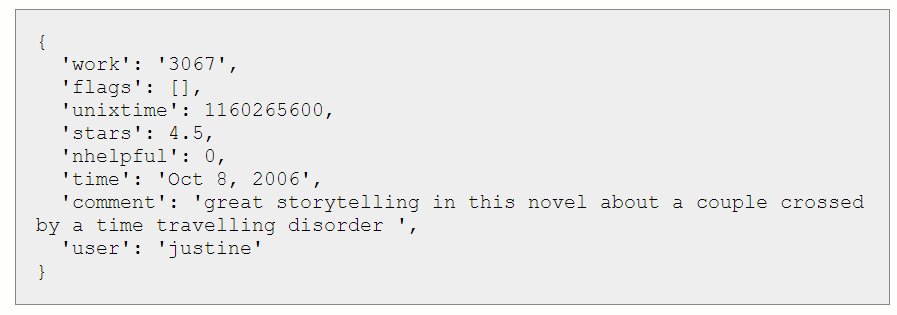
\includegraphics[scale = .7]{images/data_img.png}
    \caption{Giá trị một bản ghi dữ liệu.}
\end{figure}

Dữ liệu cho mô hình bao gồm 3 trường là người dùng, sách và đánh giá.
Kích cỡ của dữ liệu gồm 1387209 bản ghi. Ta tiến hành tiền xử lí dữ liệu, lọc ra những người dùng có lượng đánh giá lớn hơn 10 cuốn sách, để tiết kiệm thời gian huấn luyện mô hình và bộ nhớ. Sau đó dữ liệu được chia thành 2 tập là tập Train và tập Validation. Với tập Validation chiếm 5\% tập dữ liệu ban đầu, tập Train chiếm 95\% dùng cho việc học mô hình.
\begin{figure}[H]
    \centering
    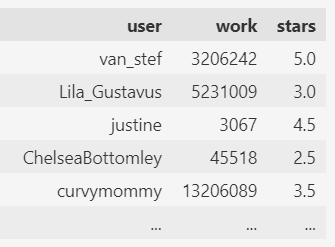
\includegraphics{images/Screenshot 2022-07-30 181900.png}
    \caption{Dữ liệu huấn luyện mô hình.}
\end{figure}

\subsubsection{Chương trình lập trình}
Mã nguồn chương trình được viết bằng ngôn ngữ lập trình Python. Chương trình bao gồm các hàm có chức năng sau:
\begin{itemize}
    \item Hàm \textit{normalize\_data()}: hàm làm chuẩn hóa dữ liệu, đưa dữ liệu về dạng chuẩn hóa.
    \item Hàm \textit{loss()}: tính giá trị hàm mất mát của mô hình.
    \item Hàm \textit{get\_items\_rated\_by\_user()}: hàm trả về các ID các cuốn sách được người đánh giá bởi 1 người dùng.
    \item Hàm \textit{get\_users\_who\_rate\_item()}: hàm trả về các ID người đọc đã đánh giá cuốn sách đó.
    \item Hàm \textit{update\_Q()}: cập nhật ma trận $Q$.
    \item Hàm \textit{update\_P()}: cập nhật ma trận $P$.
    \item Hàm \textit{fit()}: chức năng huấn luyện mô hình với dữ liệu.
    \item Hàm \textit{evaluate\_RMSE()}: đánh giá mô hình bằng phương pháp RMSE.
    \item Hàm \textit{pred()}: hàm dự đoán xếp hạng của dữ liệu được đưa vào.
\end{itemize}
Hàm \textit{fit()} được viết như sau:
\begin{lstlisting}
def fit(self):
        self.normalize_data()
        for it in range(self.Max_iter):
            self.update_Q()
            self.update_P()
            if (it + 1) % self.print_every == 0:
                rmse_train = self.evaluate_RMSE(self.Y_data)
                rmse_val = self.evaluate_RMSE(self.Y_val_set)
                print ('iter =', it + 1, ', loss =', self.loss(), ', RMSE train =', rmse_train, ', RMSE val = ', rmse_val)
            if self.loss() <=0.01:
                break
\end{lstlisting}
Ở mỗi vòng lặp chúng ta sẽ thực hiện cập nhật các tham số trong ma trận $P$ và $Q$ để tiến đến kết quả tối ưu.
\subsubsection{Kết quả thực nghiệm}
Kết quả thực nghiệm với các siêu tham số như sau:
\begin{table}[H]
    \centering
    \begin{tabular}{|c|c|c|c|c|}
    \hline
         f&$\lambda$ & $\eta$ & RMSE Train & RMSE Val \\ \hline
         10&0 & 2.5 &  1.3331 & 1.4696\\  \hline
    \end{tabular}
    \caption{Kết quả huấn luyện mô hình.}
    \label{kq}
\end{table}
\newpage
\begin{figure}[H]
    \centering
    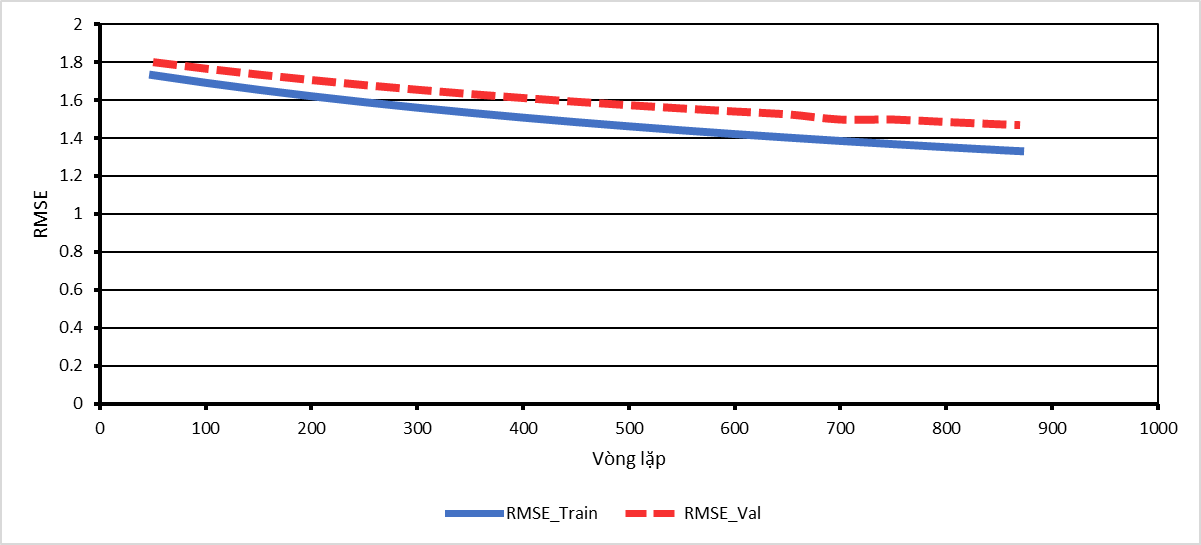
\includegraphics[scale = .8]{images/Picture1.png}
    \caption{Đánh giá RMSE qua các vòng lặp.}
    \label{rmse}
\end{figure}
Sau nhiều lần huấn luyện mô hình, kết quả ở bảng \ref{kq} là giá trị khả quan nhất, với giá trị nhân tố ẩn $f=10$ và tốc độ học $\eta= 2.5$, giá trị RMSE trên tập Train và tập Val xấp xỉ gần bằng nhau. Điều đó cho thấy mô hình của chúng ta đang không bị học quá khớp, nhưng giá trị RMSE vẫn còn khá lớn, mô hình học các tham số chưa đủ tốt và cần phải huấn luyện mô hình tốt hơn nữa bằng việc thử các tham số phù hợp.\\
Hình \ref{rmse} cho ta thấy tốc độ giảm của giá trị RMSE trên cả 2 tập Train và tập Val còn chậm. Cần cải thiện mô hình bằng cách thử các siêu tham số khác nhau về tốc độ học, để tốc độ hội tụ nhanh hơn.
\chapter{KẾT LUẬN}
\section{Kết luận}
\subsection*{Đồ án đã đạt mục tiêu đề ra}
Đồ án đã đưa ra được những khái niệm cơ bản về lĩnh vực học máy - Machine Learning. Hiểu biết bản chất của vấn đề học máy và các hướng phát triển trong tương lai. Đã tìm hiểu và nghiên cứu bài toán hệ thống gợi ý và áp dụng vào thuật toán cụ thể.
\subsection*{Kết quả đạt được}
\begin{enumerate}
    \item Trình bày rõ ràng, tổng quát khái niệm, kiến thức về lĩnh vực học máy - Machine learning.
    \item Nhận biết các vấn đề tồn tại trong bài toán hệ thống gợi ý.
    \item Trình bày thuật toán cụ thể cho bài toán hệ thống gợi ý.
    \item Có chương trình thực nghiệm kết quả.
\end{enumerate}
\subsection*{Kỹ năng đạt được khi thực hiện đồ án}
\begin{enumerate}
    \item Kỹ năng đọc và tìm hiểu các bài báo khoa học, tài liệu chuyên ngành liên quan đến nội dung của đồ án.
    \item Biết cách hệ thống nội dung, trình bày khoa học các vấn đề liên quan.
    \item Xây dựng một chương trình về học máy.
\end{enumerate}
\section{Hướng phát triển đề tài trong tương lai}
\begin{enumerate}
    \item Tìm hiểu thuật toán và xây dựng chương trình cho bài toán khi có sự xuất hiện các người dùng mới hoặc sản phẩm mới trong hệ thống gợi ý.
    \item Cập nhật yếu tố thời gian có tác động đến hệ thống gợi ý.
    \item Cải thiện mô hình với phương pháp Demographic Filtering (DF).
\end{enumerate}

\chapter*{DANH MỤC THAM KHẢO}
\addcontentsline{toc}{chapter}{DANH MỤC THAM KHẢO}
\section*{Tiếng Việt}
\begin{enumerate}
    \item Vũ Hữu Tiệp, \textit{Machine Learning cơ bản.}
\end{enumerate}
\section*{Tiếng Anh}
\begin{enumerate}
    \item Ismail Ahmed Al-Qasem Al-Hadi, Nurfadhlina Mohd SharefMd Nasir Sulaiman and Norwati Mustapha, "Review of the Temporal Recommendation System with Matrix Factorization", \textit{International Journal of Innovative Computing, Information and Control}, Vol 13;(5), 2017, pp 1579-1594.
    \item Iateilang Ryngksai and L. Chameikho, "Recommender Systems: Types of Filtering Techniques", \textit{International Journal of Engineering Research & Technology (IJERT)}, Vol 3;(11), 2014.
    \item Yehuda Koren, Robert Bell and Chris Volinsky, "Matrix factorization techniques for recommender systems", \textit{Computer (Long. Beach. Calif.)}, Vol 42;(8), 2009, pp.42-49.
\end{enumerate}